% ****** Start of file aipsamp.tex ******
%
%   This file is part of the AIP files in the AIP distribution for REVTeX 4.
%   Version 4.1 of REVTeX, October 2009
%
%   Copyright (c) 2009 American Institute of Physics.
%
%   See the AIP README file for restrictions and more information.
%
% TeX'ing this file requires that you have AMS-LaTeX 2.0 installed
% as well as the rest of the prerequisites for REVTeX 4.1
% 
% It also requires running BibTeX. The commands are as follows:
%
%  1)  latex  aipsamp
%  2)  bibtex aipsamp
%  3)  latex  aipsamp
%  4)  latex  aipsamp
%
% Use this file as a source of example code for your aip document.
% Use the file aiptemplate.tex as a template for your document.
\documentclass[%
 aip,
% jmp,
% bmf,
% sd,
% rsi,
 amsmath,amssymb,
%preprint,%
 reprint,%
%author-year,%
%author-numerical,%
% Conference Proceedings
]{revtex4-1}

\usepackage{graphicx}% Include figure files
\usepackage{dcolumn}% Align table columns on decimal point
\usepackage{bm}% bold math
%\usepackage[mathlines]{lineno}% Enable numbering of text and display math
%\linenumbers\relax % Commence numbering lines

\usepackage[utf8]{inputenc}
\usepackage[T1]{fontenc}
\usepackage{mathptmx}
\usepackage{etoolbox}

%% Apr 2021: AIP requests that the corresponding 
%% email to be moved after the affiliations
\makeatletter
\def\@email#1#2{%
 \endgroup
 \patchcmd{\titleblock@produce}
  {\frontmatter@RRAPformat}
  {\frontmatter@RRAPformat{\produce@RRAP{*#1\href{mailto:#2}{#2}}}\frontmatter@RRAPformat}
  {}{}
}%
\makeatother
\begin{document}

\preprint{AIP/123-QED}

\title[Sample title]{Sample Title:\\with Forced Linebreak}
% Force line breaks with \\
\author{A. Author}
 \altaffiliation[Also at ]{Physics Department, XYZ University.}%Lines break automatically or can be forced with \\
\author{B. Author}%
 \email{Second.Author@institution.edu.}
\affiliation{ 
Authors' institution and/or address%\\This line break forced with \textbackslash\textbackslash
}%

\author{C. Author}
 \homepage{http://www.Second.institution.edu/~Charlie.Author.}
\affiliation{%
Second institution and/or address%\\This line break forced% with \\
}%

\date{\today}% It is always \today, today,
             %  but any date may be explicitly specified

\begin{abstract}
An article usually includes an abstract, a concise summary of the work
covered at length in the main body of the article. It is used for
secondary publications and for information retrieval purposes. 
\end{abstract}

\maketitle

\begin{quotation}
The ``lead paragraph'' is encapsulated with the \LaTeX\ 
\verb+quotation+ environment and is formatted as a single paragraph before the first section heading. 
(The \verb+quotation+ environment reverts to its usual meaning after the first sectioning command.) 
Note that numbered references are allowed in the lead paragraph.
%
The lead paragraph will only be found in an article being prepared for the journal \textit{Chaos}.
\end{quotation}

\section{Introduction}
Current~\cite{girshick2014rich} state-of-the-art object detectors are based on
a two-stage, proposal-driven~\cite{lin2017focal} mechanism. As popularized
in the R-CNN framework, the first stage generates a
sparse set of candidate object locations and the second stage
classifies each candidate location as one of the foreground
classes or as background using a convolutional neural network. Through a sequence of advances , this
two-stage framework consistently achieves top accuracy on
the challenging COCO benchmark.
Despite the success of two-stage detectors, a natural
question to ask is: could a simple one-stage detector achieve
similar accuracy? One stage detectors are applied over a
regular, dense sampling of object locations, scales, and aspect ratios. Recent work on one-stage detectors, such as
YOLO and SSD, demonstrates promising
results, yielding faster detectors with accuracy within 10-
40\% relative to state-of-the-art two-stage methods.

Current~\cite{girshick2014rich} state-of-the-art object detectors are based on
a two-stage, proposal-driven~\cite{lin2017focal} mechanism. As popularized
in the R-CNN framework, the first stage generates a
sparse set of candidate object locations and the second stage
classifies each candidate location as one of the foreground
classes or as background using a convolutional neural network. Through a sequence of advances , this
two-stage framework consistently achieves top accuracy on
the challenging COCO benchmark.
Despite the success of two-stage detectors, a natural
question to ask is: could a simple one-stage detector achieve
similar accuracy? One stage detectors are applied over a
regular, dense sampling of object locations, scales, and aspect ratios. Recent work on one-stage detectors, such as
YOLO and SSD, demonstrates promising
results, yielding faster detectors with accuracy within 10-
40\% relative to state-of-the-art two-stage methods.

\section{Related Work}
\subsection{Classic Object Detectors}
\begin{figure}
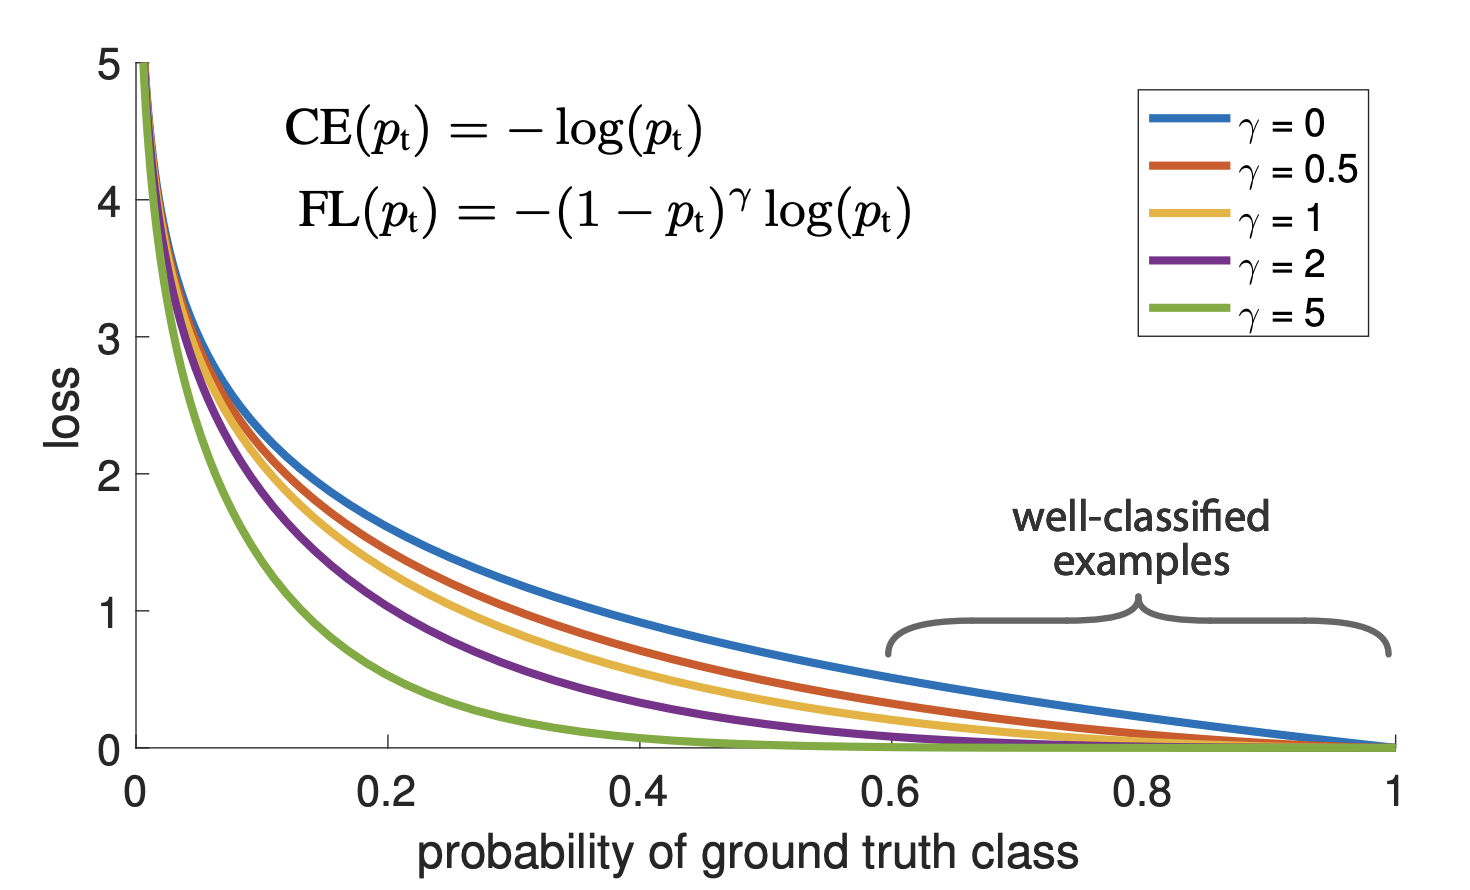
\includegraphics[width=0.4\textwidth]{Illustrations/loss.png}% Here is how to import EPS art
\caption{We propose a novel loss we term the Focal Loss that adds a factor}
\label{fig:my_label}
\end{figure}

The sliding-window paradigm (Fig.~\ref{fig:my_label}),
in which a classifier is applied on a dense image grid, has
a long and rich history. One of the earliest successes is the
classic work of LeCun et al. who applied convolutional neural networks to handwritten digit recognition (Equation~\ref{eq_1}). Viola and Jones [36] used boosted object detectors for face
detection, leading to widespread adoption of such models.
The introduction of HOG [4] and integral channel features
[5] gave rise to effective methods for pedestrian detection.
DPMs [8] helped extend dense detectors to more general
object categories and had top results on PASCAL [7] for
many years. While the sliding-window approach was the
leading detection paradigm in classic computer vision, with
the resurgence of deep learning [17], two-stage detectors,
described next, quickly came to dominate object detection.

% \begin{figure}
%     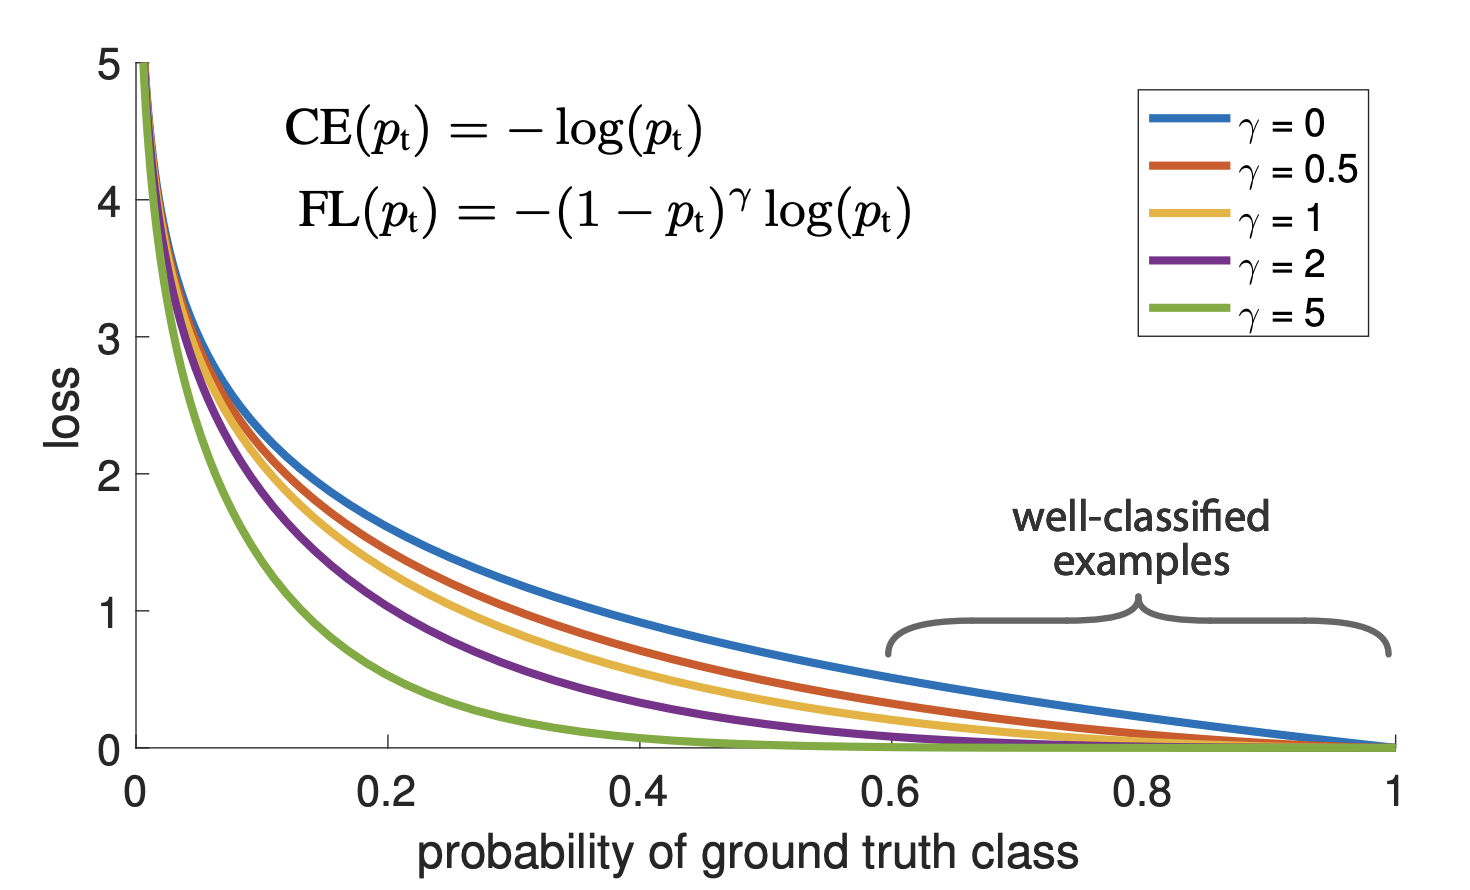
\includegraphics{Illustrations/loss.png}
%     \caption{We propose a novel loss we term the Focal Loss that adds a factor}
%     \label{fig:my_label}
% \end{figure}

Two-stage Detectors: The dominant paradigm in modern
object detection is based on a two-stage approach. As pioneered in the Selective Search work [34], the first stage generates a sparse set of candidate proposals that should contain all objects while filtering out the majority of negative
locations, and the second stage classifies the proposals into
foreground classes / background. R-CNN (Equation~\ref{eq:CE}) upgraded the
second-stage classifier to a convolutional network yielding
large gains in accuracy and ushering in the modern era of
object detection. R-CNN was improved over the years, both
in terms of speed [14, 10] and by using learned object proposals [6, 23, 27]. Region Proposal Networks (RPN) integrated proposal generation with the second-stage classifier
into a single convolution network, forming the Faster RCNN framework [27]. Numerous extensions to this framework have been proposed, e.g.




% \begin{figure}
% 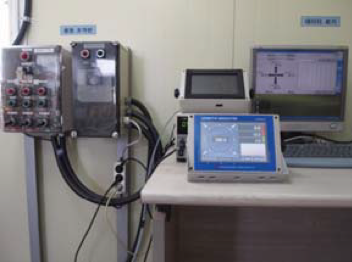
\includegraphics{fig_1}% Here is how to import EPS art
% \caption{\label{fig:epsart} A figure caption. The figure captions are
% automatically numbered.}
% \end{figure}
% is small enough to fit in a single column, while
% Fig.~\ref{fig:wide}%
% \begin{figure*}
% \includegraphics{fig_2}% Here is how to import EPS art
% \caption{\label{fig:wide}Use the \texttt{figure*} environment to get a wide
% figure, spanning the page in \texttt{twocolumn} formatting.}
% \end{figure*}

\begin{equation}\label{eq_1}
\boxed{Ax=b}
\end{equation}

\begin{equation}
\operatorname{FL}\left(p_{\mathrm{t}}\right)=-\left(1-p_{\mathrm{t}}\right)^\gamma \log \left(p_{\mathrm{t}}\right)
\end{equation}

\begin{equation}\label{eq:CE}
\mathrm{CE}(p, y)= \begin{cases}-\log (p) & \text { if } y=1 \\ -\log (1-p) & \text { otherwise }\end{cases}
\end{equation}


\newpage

\nocite{*}
\bibliography{aipsamp}% Produces the bibliography via BibTeX.

\end{document}
%
% ****** End of file aipsamp.tex ******